\documentclass[main]{subfiles}

\begin{document}

\begin{frame}
\frametitle{Chaotic Systems}
\begin{enumerate}
\visible<2->{
\item \textbf{Chaotic system} is a \textbf{non-linear, dynamical system} exhibiting chaotic dynamics.
}
\visible<3->{
\item Chaos means that even in a deterministic system, where the future behavior is fully determined by the initial state, a slightly varied initial state makes the system unpredictable.
}
\visible<4->{
\item A chaotic system must..\footnotemark
\begin{itemize}
\item be sensitive to the initial conditions.
\item show topological mixing.
\item have dense periodic orbits.
\end{itemize}
\footnotetext{R. L. Devaney - An Introduction to chaotic dynamical systems (1989)}
}
\end{enumerate}
\end{frame}

\begin{frame}
\begin{figure}[H]
\centering
\includegraphics[scale=0.75]{controllers/sinusoid-controller.pdf}

\caption[The sinusoid controller]{The specification of the sinusoid controller, its internal state and output signal. The internal state has the same dimensionality as the output. If the sinusoidal controller is mutated during the mutation step of the simulator, the parameters are chosen from a uniform distribution over the respective intervals.}
\label{figure:sinusoid-controller}
\end{figure}
\end{frame}

\begin{frame}
\begin{figure}[H]
\centering
\includegraphics[width=0.49\textwidth]{controllers/chua-circuit/Chua-circuit-with-chua-diode.pdf}
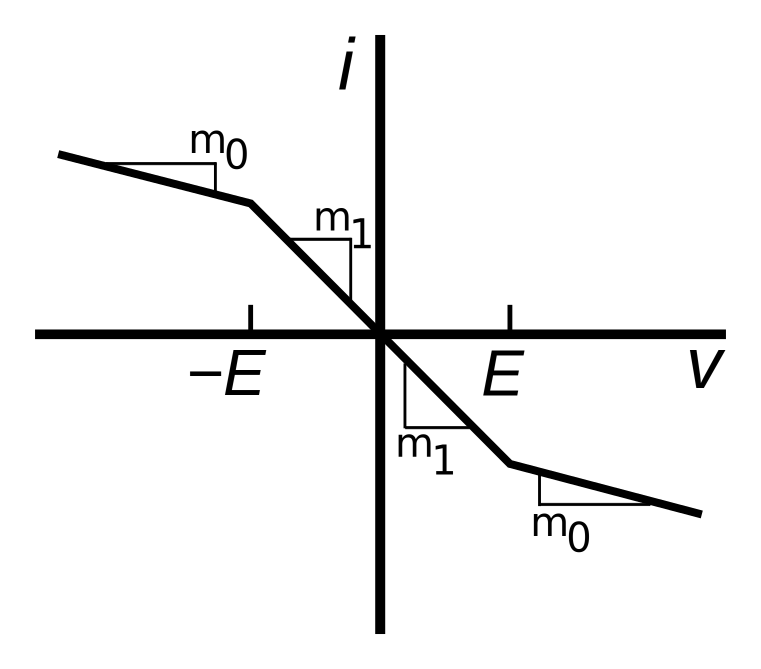
\includegraphics[width=0.49\textwidth]{controllers/chua-circuit/Chua-diode-characteristic-curve.pdf}
\caption[The Chua circuit]{The Chua circuit with its special Chua diode. The Chua diode is a piecewise-linear resistor with the characteristics as shown in the right figure.}
\label{figure:chuacircuit}
\end{figure}
\end{frame}

\begin{comment}
\begin{frame}

  \frametitle{Contents}
  \tableofcontents[currentsection]
\end{frame}


\section{Something}

\frame{

  \frametitle{Evolving Virtual Creatures}
  
  \begin{columns}
   \column{0.3\textwidth}
 \begin{itemize}
	     \item a
    	\item b
    	\item c
     \end{itemize}
     
     \column{0.6\textwidth}
      %\includegraphics[width=2in, clip] {figs/creatures.jpg} 
  \end{columns}
  }
\note{}

\begin{frame}
\textbf{New colors and their names\\}
Here we show the different colors you can use. From left to right, this are the colors ETH1, ETH2, \ldots , ETH9.

\newcommand{\quadrat}{(0,0mm)--(0mm,5mm)--(5mm,5mm)--(5mm,0mm)--(0mm,0mm);}
\begin{center}
	\hspace{-8mm}
	\begin{tikzpicture}[overlay]
		{\draw[ETHa,fill=ETHa] \quadrat}\label{ETH1}
	\end{tikzpicture}
	\hspace{10mm}
	\begin{tikzpicture}[overlay]
		{\draw[ETHb,fill=ETHb]\quadrat}\label{ETH2}
	\end{tikzpicture}
	\hspace{10mm}
	\begin{tikzpicture}[overlay]
		{\draw[ETHc,fill=ETHc]\quadrat}\label{ETH3}
	\end{tikzpicture}
	\hspace{10mm}
	\begin{tikzpicture}[overlay]
		{\draw[ETHd,fill=ETHd] \quadrat}\label{ETH4}
	\end{tikzpicture}
	\hspace{10mm}
	\begin{tikzpicture}[overlay]
		{\draw[ETHe,fill=ETHe] \quadrat}\label{ETH5}
	\end{tikzpicture}
	\hspace{10mm}
	\begin{tikzpicture}[overlay]
		{\draw[ETHf,fill=ETHf] \quadrat}\label{ETH6}
	\end{tikzpicture}
	\hspace{10mm}
	\begin{tikzpicture}[overlay]
		{\draw[ETHg,fill=ETHg] \quadrat}\label{ETH7}
	\end{tikzpicture}
	\hspace{10mm}
	\begin{tikzpicture}[overlay]
		{\draw[ETHh,fill=ETHh] \quadrat}\label{ETH8}
	\end{tikzpicture}
	\hspace{10mm}
	\begin{tikzpicture}[overlay]
		{\draw[ETHi,fill=ETHi] \quadrat}\label{ETH9}
	\end{tikzpicture}
\end{center}

Please use no more then two of them in your presentation. The first two (counted from the left hand side) are reserved for the administration chapter of the ETHZ (first one for external presentation, second for internal), all others you can freely choose.

\end{frame}

\begin{frame}
\textbf{Some mathematical specialities}

\ETHbox{0.8\textwidth}{% define the ETHbox
  \begin{theorem}[Murphy (1949)]\label{murphy}
    Anything that can go wrong, will go wrong.
  \end{theorem}
}

\begin{proof}
  A special case of Theorem \ref{murphy} is proven in %\citet{matthews1995}.
\end{proof}
\end{frame}

\begin{titlestyleframe}
\frametitle{Title Page}

\color{white} The title page is created using the \texttt{\textbackslash titleframe} command.

The title page background can also be used on other frames (or for a customised title frame) using the \texttt{titlestyleframe} environment.
\end{titlestyleframe}

\begin{frame}
\frametitle{Normal Frame}
The normal frame looks like this. It is created using the \texttt{frame} environment.
\end{frame}

\begin{inverseframe}
  \frametitle{Inverse Slides}
  %\color{white}
The inverted frame looks like this. It is created using the \texttt{inverseframe} environment.
\end{inverseframe}

\begin{minimalframe}
  \frametitle{Minimal Frame}
The minimal frame looks like this. It is created using the \texttt{minimalframe} environment.
  
\end{minimalframe}

\end{comment}

\end{document}